\chapter{Pipeline and Results}
This chapter introduces a pipeline of the \textit{in silico} data set (Figure 3.3) and a pipeline for the DREAM8 Challenge data set (Figure 3.8) describing the processing of the data from discretization to inferring a network and finally scoring the predicted network against a gold standard network. The results of the \textit{in silico} data set are necessary to set the parameter for the DREAM8 Challenge pipeline. Both pipelines can be executed from the command line by a bash script and are available on Git: "github.com/ninakersten/Masterthesis". 

\section{Pipeline of the \textit{in silico} data set}

For both the sub-networks of \textit{E.coli} and the cell cycle network each set $F$ of transition function is executed to sets of continuous data ($S=\{ S_{1},S_{2},...,S_{n}\} $), which are generated with \textit{odefy}, a MATLAB- and Octave-compatible toolbox for the automated transformation of Boolean models into systems of ordinary differential equations %\citep{Krumsiek2010}
(Figure 3.3, Figure 3.1). With \textit{odefy} the number of sample points and the time interval for a data simulation can be determined. The time interval is set to a range of 1 to 50. The \textit{in silico} data sets are converted into the \textit{csv} format of the structure of the DREAM8 Challenge input data (Table 2.1) and for the discretization and learning step converted into a \textit{text} file format (Figure 3.1). Names of the species are anonymized by single characters depicted in the first header of a \textit{txt} file and original names are stored in a header below followed by the time course data set \textit{S}. Information about cell line, inhibitor and stimulus are neglected (Figure 3.1).

%\noindent See the following command :
%\begin{lstlisting}[language=bash]
%  $ bash insilico.sh 100 KM3 BESTFIT
%\end{lstlisting}

%bild zeigen, wie die Daten in dem file angeordnet sind.
\begin{figure}[H]
\captionsetup{width=0.9\linewidth}
\centering
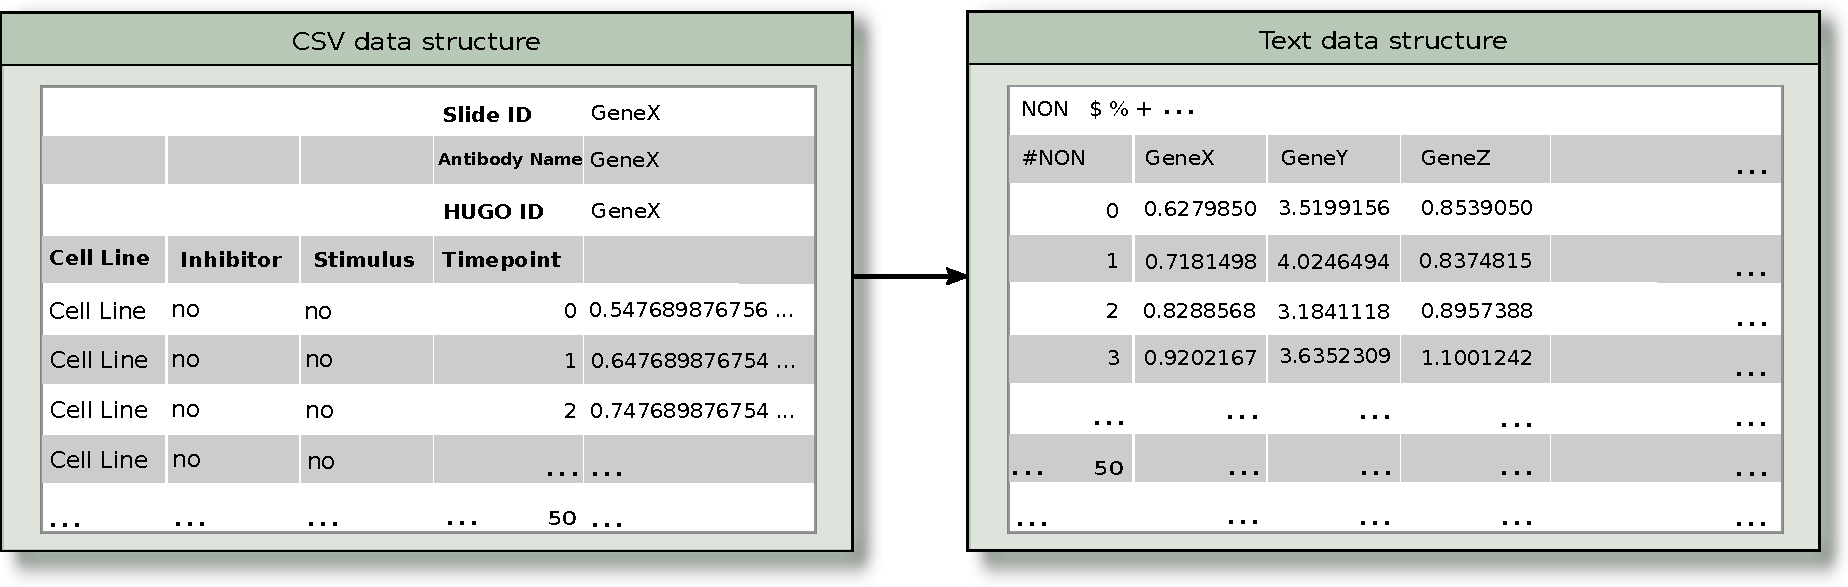
\includegraphics[width=1.0\textwidth]{./Bilder/CSV2TXT.pdf}
\caption[$CSV$ to $TXT$]{\textbf{$CSV$ to $TXT$:} Anonymized single character represent the species and information about cell line, inhibitor and stimulus is neglected. }
\label{fig:9}
\end{figure}

\newpage
After discretizing continuous time course data into a set of binary values ($B=bin(S)$, where $bin\in \{ $2-\textit{k-means}, iterative \textit{k-means}$\}$) redundant values are removed from this set. Boolean networks ($N=learn(B)$) are learned from this data by each inference algorithm ($learn\in \{$Best-Fit, Full-Fit, Reveal$\}$). A value for the minimal error $MinError$ is set, such that an inference algorithm runs i times (here: $i=5000$) until a network with an error ($Error(N,B)$) lower than the minimal error is achieved. 
%  Den Value für minimalen Error hier angeben= 10!!!!!
It is worthwhile to get an error of $0$, meaning the Boolean model describes the data perfectly. The amount of returned solutions is set to a value of $3$, such that in each inference process three solutions (resp. Boolean Networks) are inferred, all with an error lower than the minimal error. A single Boolean Network with the lowest error across all iterations is selected for further structural evaluation.
\subsection*{Inference settings}
For investigating the impact of the \textit{in-degree} in a network on the algorithms performance, sub-networks of \textit{E.coli} are processed by the iterative \textit{k-means} binarization algorithm with a cluster depth of $d=3$ in combination with Best-Fit, Full-Fit or REVEAL. The cluster depth with $d=3$ is selected due to previous research proving its reliability regarding the trade-off between simplicity and loss of information (e.g. oscillations).\\
\citep{Berestovsky.2013}
For assessing the dependence of an inference algorithm to the number of sample points, continuous data for the cell cycle is generated for $m\in\{ 50$, $100$, $150$, $200$, $250$, $300$, $350$, $400$ ,$450$, $500\}$. 
The whole set of inference algorithms only runs starting by 50 sample points. Complex systems, like a cell cycle are oscillating, thus a large number of sample points are needed to detect 'real' steady-states and achieve a sufficient Boolean network.\\

For measuring the impact of the clustering depth the cell cycle's continous data is generated with 100 sample points (similar to the abundance of sample points of $\sim 85$ in the DREAM8 Challenge) and inferred with a clustering depth of $d\in \{ 1,2,3,4,5,6,7,8,9,10\}$, where $d=1$ denote the two clusters \textit{k-means} binarization algorithm and from $d=2$ denote the iterative \textit{k-means} binarization algorithm. Table 3.1 shows a summarized overview of the settings for the \textit{in silico} pipeline.
%Hiernoch angeben, dass iterative k-means = d = 3
%und 2-k-means = d = 2
\begin{table}[H]
%\resizebox{\textwidth}{!}{
%{\tabcolsep=6pt%
\begin{center}
%\captionsetup{width=0.87\linewidth}
%\small
\scriptsize
\begin{tabular}{l|c|c|c}
\toprule 
Settings: Pipeline & \textit{in-degree} & sample points & cluster depth ($k$) \\
 \hline\hline
\# sample points & 100 & $[50:500]$ & 100 \\
\rowcolor{black!10} time interval & $[1:50]$ & $[1:50]$ & [1:50]\\
bin-method & $k=3$ & $k=3$ & $k \in [1,10]$\\
\rowcolor{black!10} REVEAL & \checkmark & \checkmark & \checkmark \\
Best-Fit & \checkmark & \checkmark & \checkmark \\
\rowcolor{black!10} Full-Fit & \checkmark & \checkmark & \checkmark \\
$MinError$ ($\epsilon$) & $0.6$ & $0.6$ &  $0.6$\\
\rowcolor{black!10} max. iteration ($i$)& 5000 & 5000 & 5000\\
solutions & 3 & 3 & 3 \\
\toprule
Network properties & & & \\
\hline\hline
\rowcolor{black!10} network source & $E.coli$ & Cell cycle & Cell cycle \\
\# networks & 45 & 10 & 10 \\
\rowcolor{black!10} max. \textit{in-degree} & $d\in [9:14]$ & 6 & 6 \\
\# nodes & $n\in [10:14]$ & 10 & 10 \\
\rowcolor{black!10} \# edges & $[10:126]$ & 35 & 35 \\
\bottomrule
\end{tabular}
\captionof{table}{Settings: Pipeline \textit{in silico} and network properties }
\end{center}
%}
\end{table}  

%!!!!!!MinError hier noch angeben!!!!!!

\subsection*{Prediction processing}

The predicted Boolean networks are converted (from \textit{.bnet}-format) into Interaction graphs (to a \textit{.sif}-format) by \textit{PyBoolNet} (Figure 3.2). Each interaction graph of a predicted network is scored against its gold standard interaction graph generated from the initial Boolean network with \textit{PyBoolNet}.\\
Hence, each line in a \textit{.sif}-file of an interaction graph represents an edge in a Boolean network (Figure 3.2). The edges of the gold standard and the prediction are compared resulting in a confusion matrix for computing precision, recall, accuracy, balanced accuracy and the Matthew correlation coefficient (Table 2.7).

\begin{figure}[H]
\centering
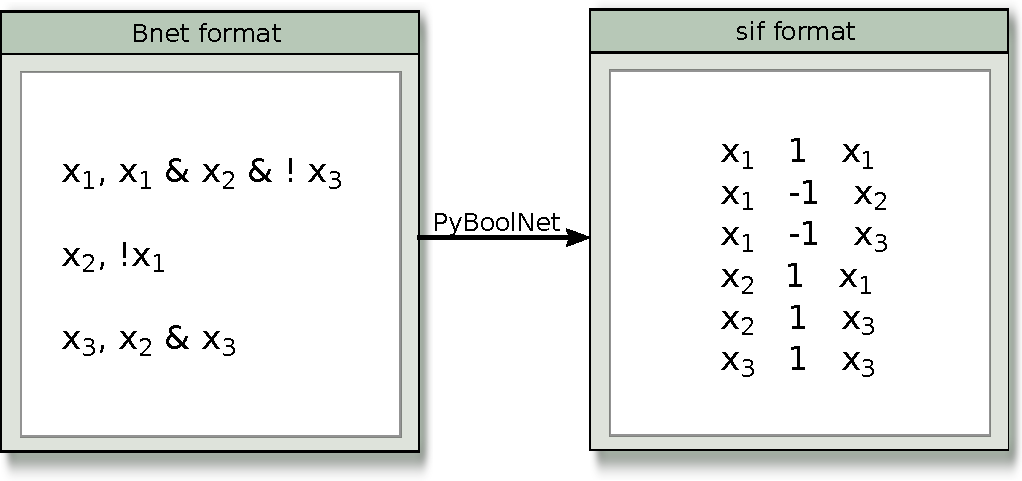
\includegraphics[width=0.7\textwidth]{./Bilder/bnet2sif.pdf}
\caption[Boolean Network to Interaction Graph]{\textbf{Boolean Network to Interaction Graph:} The predicted Boolean network $N$ (\textit{.bnet}-format) is converted into an interaction graph $IG$ (\textit{.sif}-format).}
\label{fig:9}
\end{figure}

 

\begin{figure}[H]
\centering
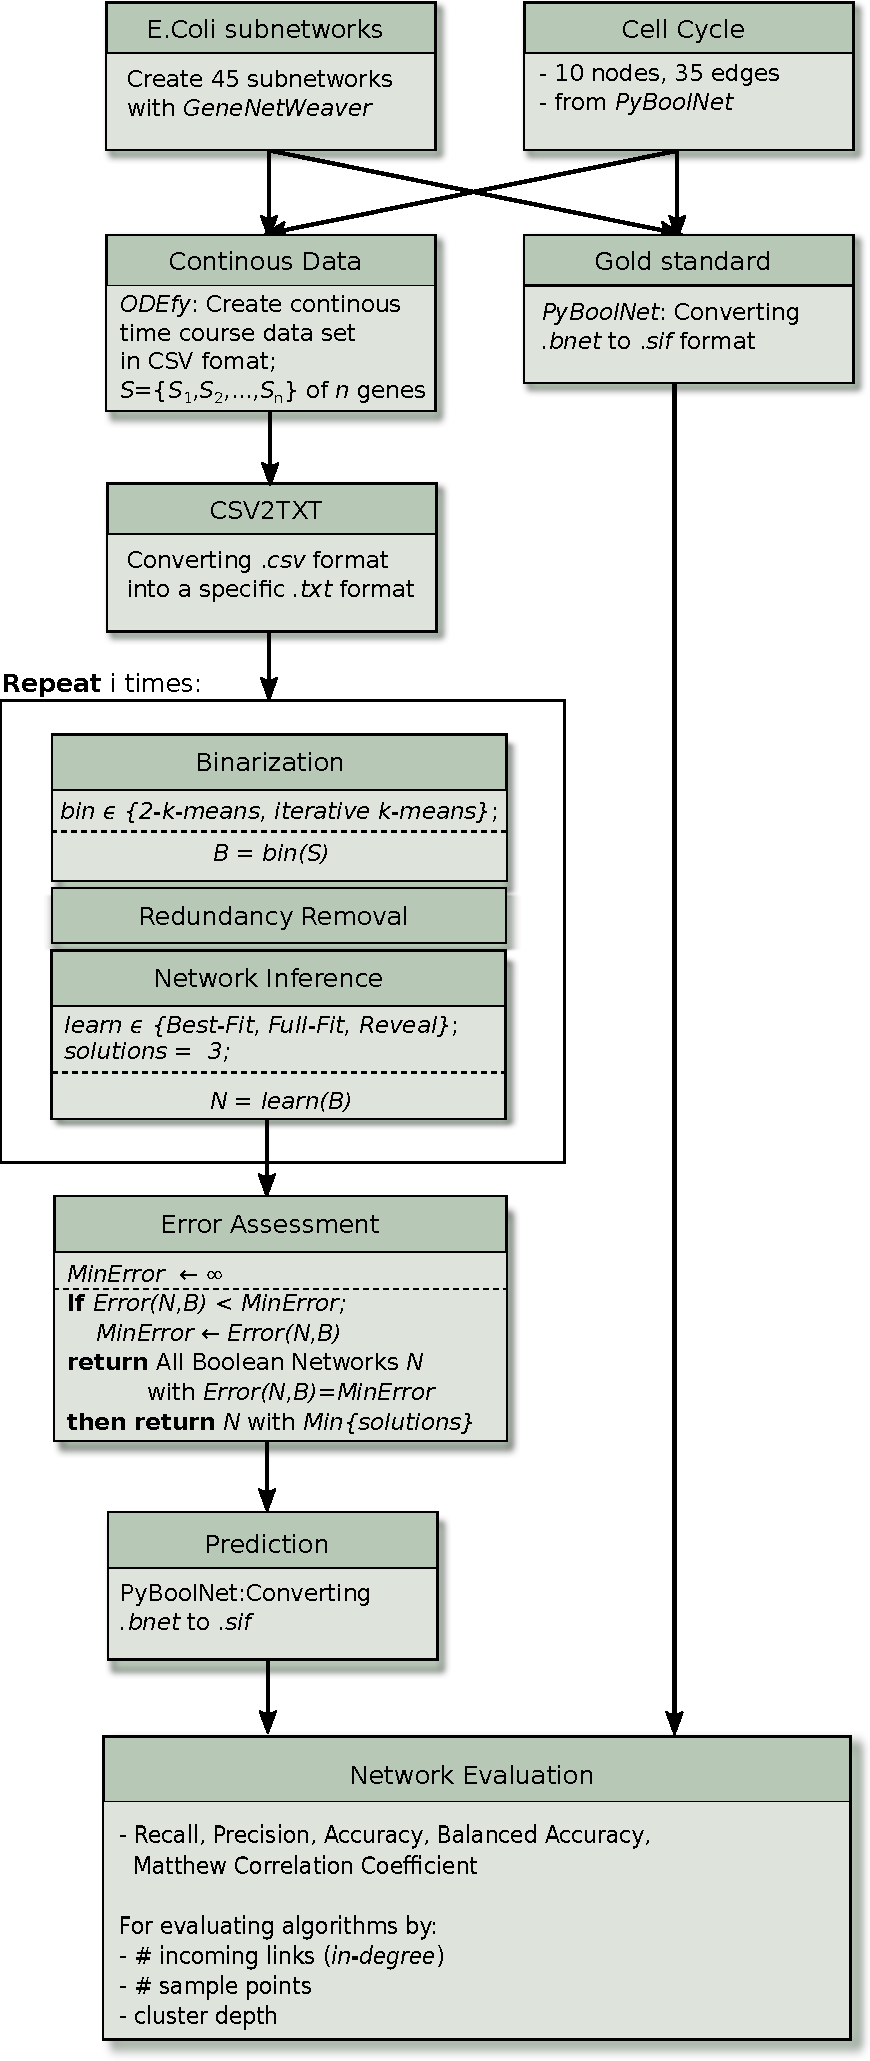
\includegraphics[width=0.55\textwidth]{./Bilder/pipeline_insilico.pdf}
\caption[Pipeline \textit{in silico}]{\textbf{Pipeline \textit{in silico}. }This pipeline shows the final setup for assessing the algorithms performance regarding the number of incoming links of nodes in a network, the number of sample points and the cluster depth for binarization.}
\label{fig:9}
\end{figure}



\section{Results and Discussion of the \textit{in silico} data set}
\subsection*{\textit{In-degree}}
Figure 3.4 shows 45 sub-networks of \textit{E.coli} grouped into nine categories, each containing five sub-networks with $n$ nodes; $n\in |V|$, where $|V|=\{10,11,12,13,14\}$. Each category on the x-axis depicts the \textit{in-degree} $k^{in}_i \in \{1,2,3,4,5,6,7, 8, 9\}$) of a set of nodes in a network. Thus, the inference algorithms Best-Fit, Full-Fit and REVEAL predict five networks in each category where the mean accuracy value is obtained by scoring each predicted interaction graph against a corresponding gold standard interaction graph, derived from the initial network $N'$ (Figure 3.3).\\
Starting with an \textit{in-degree} of $k^{in}_{1}=1$ the mean accuracy values of Best-Fit, Full-Fit and REVEAL are $\sim 0.854$, $\sim 0.844$ and $\sim 0.849$. With increasing \textit{in-degree} the mean accuracy value decreases for all three inference algorithms. Thus, with an \textit{in-degree} of $k^{in}_{9}=9$ the mean accuracy value for Best-Fit, Full-Fit and REVEAL are $\sim 0.399$, $\sim 0.407$ and $\sim 0.399$. None of the three inference algorithms show an outstanding significantly higher or lower mean accuracy. Hence, on average about $\sim 85,2\% $ of relevant links are predicted correctly by all three inference algorithms when the \textit{in-degree} is $k^{in}_{1}=1$ and an average of about $\sim 40,2\% $ of relevant links are predicted correctly by an \textit{in-degree} of $k^{in}_{9}=9$.

\begin{figure}[H]
\captionsetup{width=0.9\linewidth}
\centering
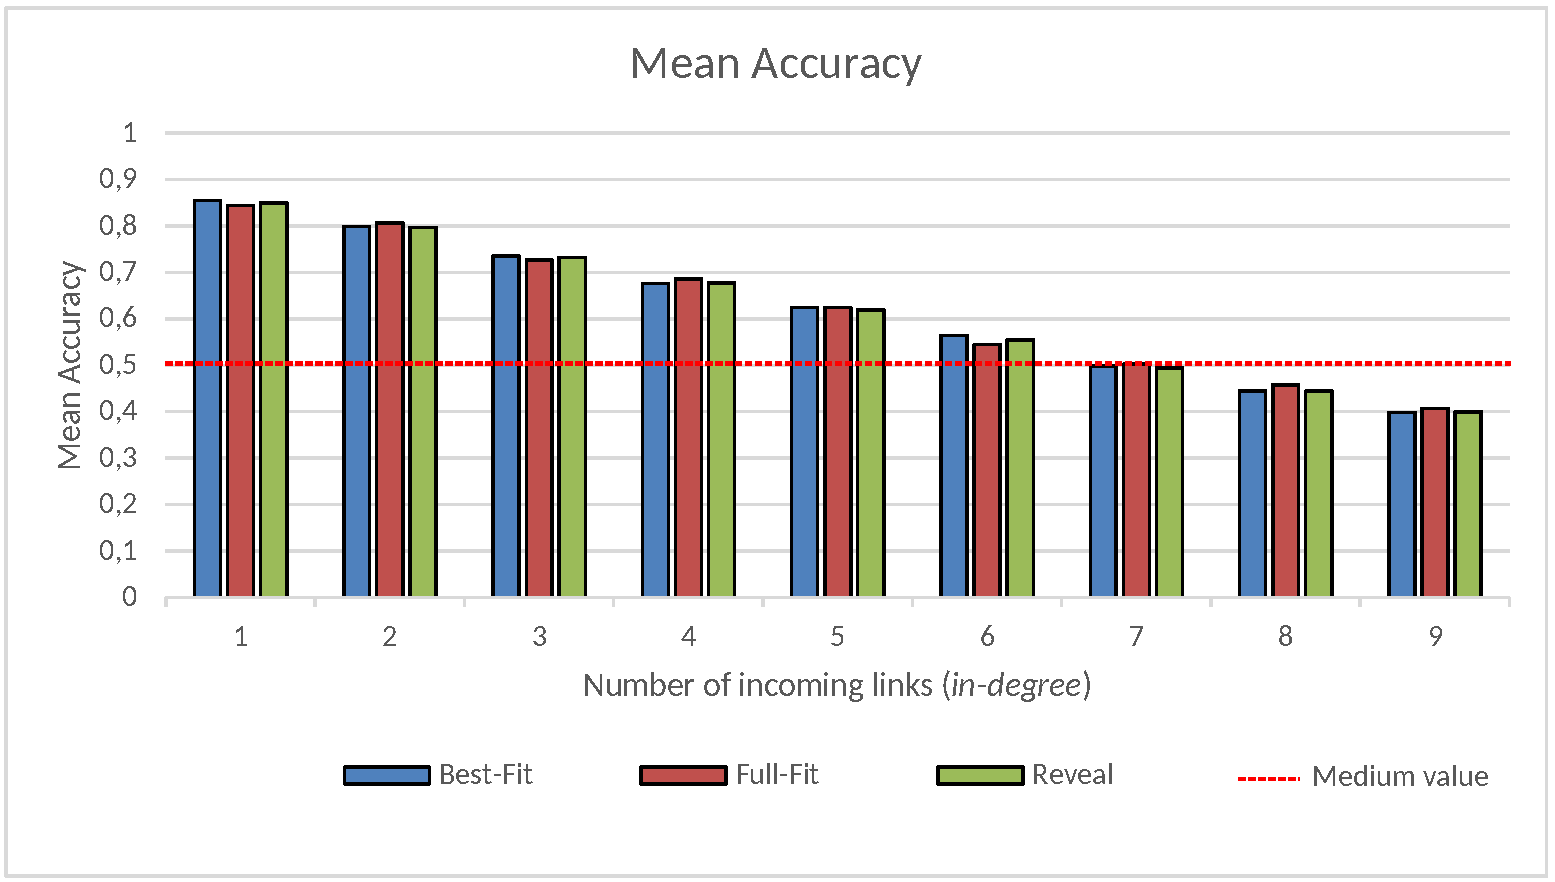
\includegraphics[width=0.9\textwidth]{./Bilder/Scoring/insilico/1_Indegree_Runtime/MeanAcc_indegree.pdf}
\caption[\textit{In-degree}:Mean Accuracy]{\textbf{\textit{In-degree}:Mean Accuracy.} Sub-networks of \textit{E.coli} are grouped into nine groups definded by the \textit{in-degree} of nodes in each sub-network. With increasing \textit{in-degree} the mean accuracy of all three inference algorithms decreases.}
\label{fig:}
\end{figure}

Thus the more nodes occur with a high \textit{in-degree} the more complex is the system and the worse the inference algorithm is able to detect the whole information. This observation captures the observation of Shohang Barman and Yung-Keun Kwon \citep{Barman.2017} who state that the number of incoming links represent the degree of complexity of the inference problem. They introduced a novel mutual information-based Boolean network inference (MIBNI) method and tested its structural and dynamic performance. Therefore, about $\sim 300$ sub-networks of \textit{E.coli} of different network sizes ($|V| = 10,20,$...$,100$) were randomly generated by $GeneNetWeaver$ and nodes of these networks were grouped by their \textit{in-degree}. Their new method yielded a slightly better performance in contrast to Best-Fit and REVEAL. Nevertheless, with incresing number of incoming links the mean accuracy decreases for all measured inference algorithms assessed in this article, too.

%Diskussion:
%- The more complex a system is (nodes have high in-degree) the more challenging it is to predict whole set dertiming a nodes state.

%\newpage
\subsection*{Number of sample points}
Continuous data sets of the mammilian cell cycle network are generated with different number of sample points $m\in \{50,100,150,200,250,300,350,400,450,500\}$ and the predicted interaction graph is scored against the interaction graph of a gold standard cell cycle interaction graph derived from the initial network (Figure 3.3).\\
In Figure 3.5 (a) recall values of Best-Fit, Full-Fit and REVEAL are ranging between $0$ (REVEAL) and $\sim 0.231$ (Best-Fit). The values fluctuate across the number of sample points for each of the three inference algorithms and regarding the overall mean recall, about $\sim 9.49\%$ of relevant links ($TP$ and $FN$) are predicted. \\
Taking the precison in Figure 3.5 (b) of Best-Fit, Full-Fit and REVEAL into account the values fluctuate among the increasing number of sample points, too. Here, values range from $0$ (REVEAL) to $\sim 0.428$ (Best-Fit). 
The mean precision value of Best-Fit is $\sim 0.236$ and for Full-Fit is $\sim 0.252$ and for REVEAL is $\sim 0.219$. \\
Thus, averaging across Best-Fit, Full-Fit and REVEAL about $\sim 23,6\% $ of the predicted links are predicted correctly.

\begin{figure}[H]
\captionsetup{width=0.9\linewidth}
\centering
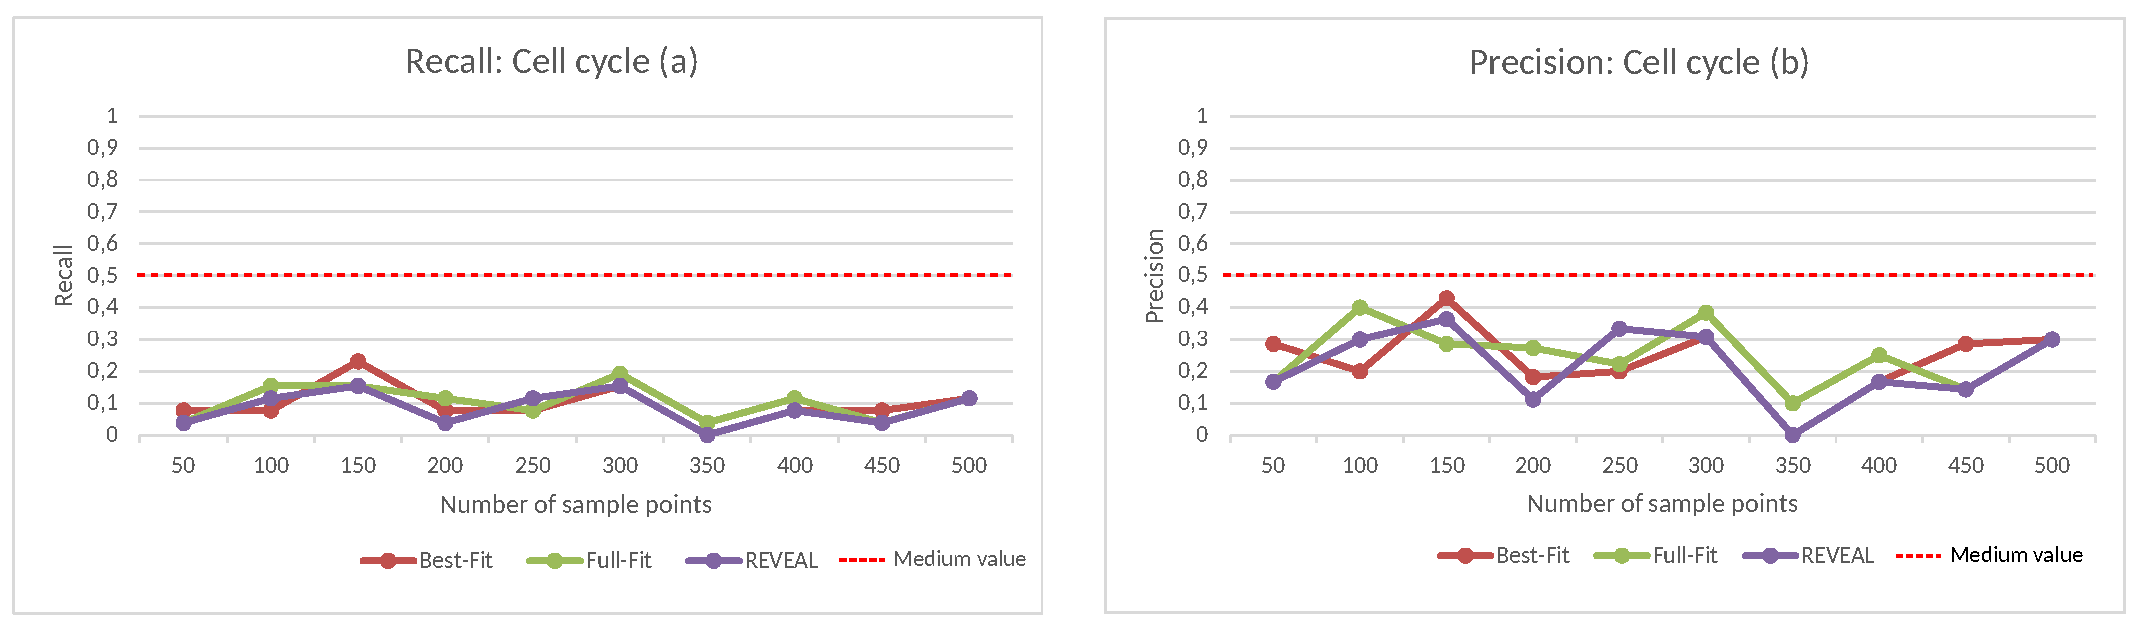
\includegraphics[width=1.0\textwidth]{./Bilder/Scoring/insilico/2_cellcycle_measurements/RecPrec.pdf}
\caption[Precision and Recall: Number of sample points]{\textbf{Number of sample points.} (a) Recall for Best-Fit, Full-Fit and REVEAL; (b) Precision for Best-Fit, Full-Fit, REVEAL}
\label{fig:}
\end{figure}
\newpage
Fluctuations across the increasing number of sample points in Figure 3.5 may be a result of the oscillating property of the cell cycle system, which is not captured in each network. The number of false negative predicted links is tremendeously high in constrast to the number of true positive predicted links for all inference algorithms, which explaines the recall. While precision is taking the true positive and false positive predicted links into account, which are not that highly class im-balanced like the classes for the recall are.\\

For this reason the balanced accuracy is considered (Figure 3.6). Here, the class imbalance is relativized, such that all three inference algorithms range around a value of $\sim 0.5$ among the increasing number of sample points. This means, each inference algorithm predicts the links in a network rather randomly. 

\begin{figure}[H]
\captionsetup{width=0.9\linewidth}
\centering
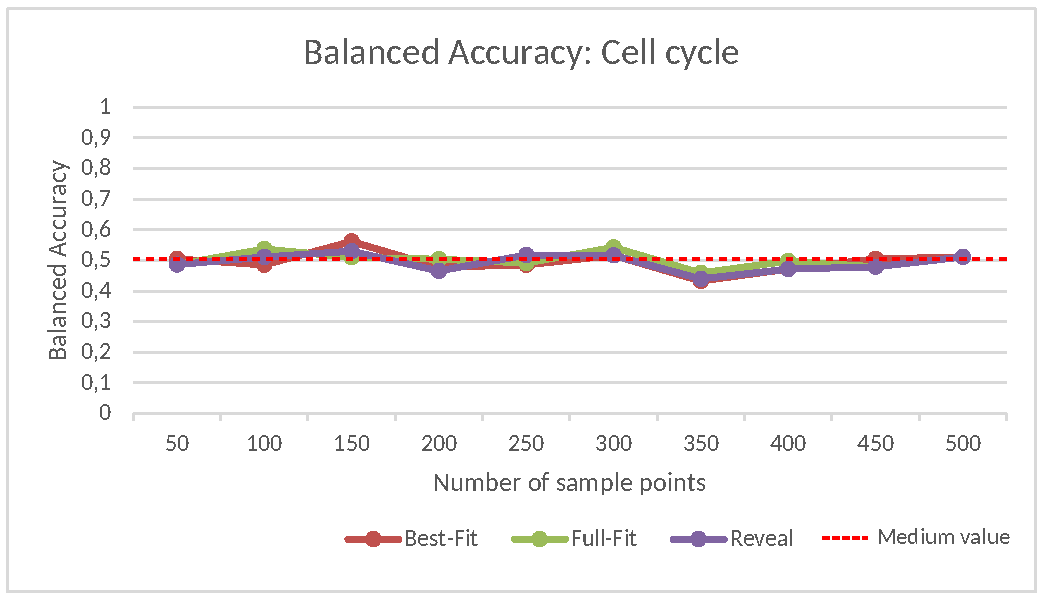
\includegraphics[width=0.9\textwidth]{./Bilder/Scoring/insilico/2_cellcycle_measurements/Bacc.pdf}
\caption[Balanced Accuracy: Number of sample points]{\textbf{Balanced Accuracy: Number of sample points.}}
\label{fig:}
\end{figure}

Regarding recall, precision and balanced accuracy in this setting context it is observed that the number of sample points has no significant impact on the inference algorithms' performance.\\
The cell cycle is with 35 links a highly interconnected network and due to its' oscillating property quite challenging to infer.
Thus, taking prior knowledge from literature into account it is important to mention, that this observation is not true for less complex networks of smaller size \citep{Berestovsky.2013}. %\citep{ "Boolean network inference from time series data incorporating prior biological knowledge" Haider and Pal BMC Genomics 2012, 13(Suppl 6):S9 http://www.biomedcentral.com/1471-2164/13/S6/S9}



%Diskussion:
%- inference algorithms are stable across the number of sample points
%- Precision: Fluctutation because of oscillating system of the cell cycle, thus in combination with the binarization method (KM=3) sometimes steady-states are detected well, low Error, and sometimes not
%-The more nodes are in a system, the more time points are needed to capture dynamics of a system
%- Meets observation of \citep{TS2B-Paper}, where with increasing number of nodes and thus, increasing complexity the number of sample point have to increase, such that tru dynamics can be captured (find a network below minError). e.g. In \textit{Jak-Stat} signal transduction pathway with 5 nodes (pJak2, pEpoR, pStat5, CIS, Socs3) with only 14 timepoints, no oscillations, but for a system of cell cycle with 10 nodes at least 30 time points are needed for Best-Fit and Full-Fit and $\sim 50$ time points are needed for REVEAL.
% Recall: Nur 10%, weil: MinError sehr groß gewählt wurde.
% Precision: Fluctering, weil cell cycle oscilating system. Binarization algorithm capture dynamics sometimes well, sometimes not. Wert gut, weil TN stark den tp überwiegen. Recall schlecht, weil FN genauso hoch wie TN und TP sehr wenig.
\newpage
\subsection*{Cluster depth}
In Figure 3.7 the cluster depth $d$ is increased from $d=1$, which represents the two clusters \textit{k-means} binarization algorithm and from $d=2$ to $d=10$ describing the cluster depth of the iterative \textit{k-means} binarization algorithm. In (a) the Matthew correlation coefficient starts with the highest value of $\sim 0.258$ for REVEAL for $d=1$ followed by Full-Fit with a value of $\sim 0.106$ and Best-Fit with $\sim 0.106$. Proceeding with $d=3$ Best-Fit stands out with a value of $\sim 0.258$ whereas Full-Fit and REVEAL range around a value of $0$. With increasing cluster depth the performance of all three inference algorithms approximates around a mean value of $\sim 0.048$.\\
In comparison with balanced accuracy in (c) when $d=3$ Best-Fit perfoms the best with a value of $0.588$ as well. Increasing the cluster depth yields an approximation of all inference algorithms around a mean value of $\sim 0.516$.\\
In (b) Best-Fit yields the best performance with a precision value of $0.6$ and  $d=3$. The value highly fluctuates until $d=5$ and approximates from $d=6$ to a precision value of $\sim 0.287$. Regarding the recall in (d) none of the inference methods is significantly outstanding. Taking the mean recall approximatly $\sim 12,3\% $ of relevant links are predicted by the methods. While $\sim 28,7\% $ of predicted links are correctly predicted.

%Overfitting:\citep{ https://doi.org/10.1371/journal.pone.0162259}

%Regarding the precision (Figure 3.7 (b)) 
\begin{figure}[H]
\captionsetup{width=1.0\linewidth}
\centering
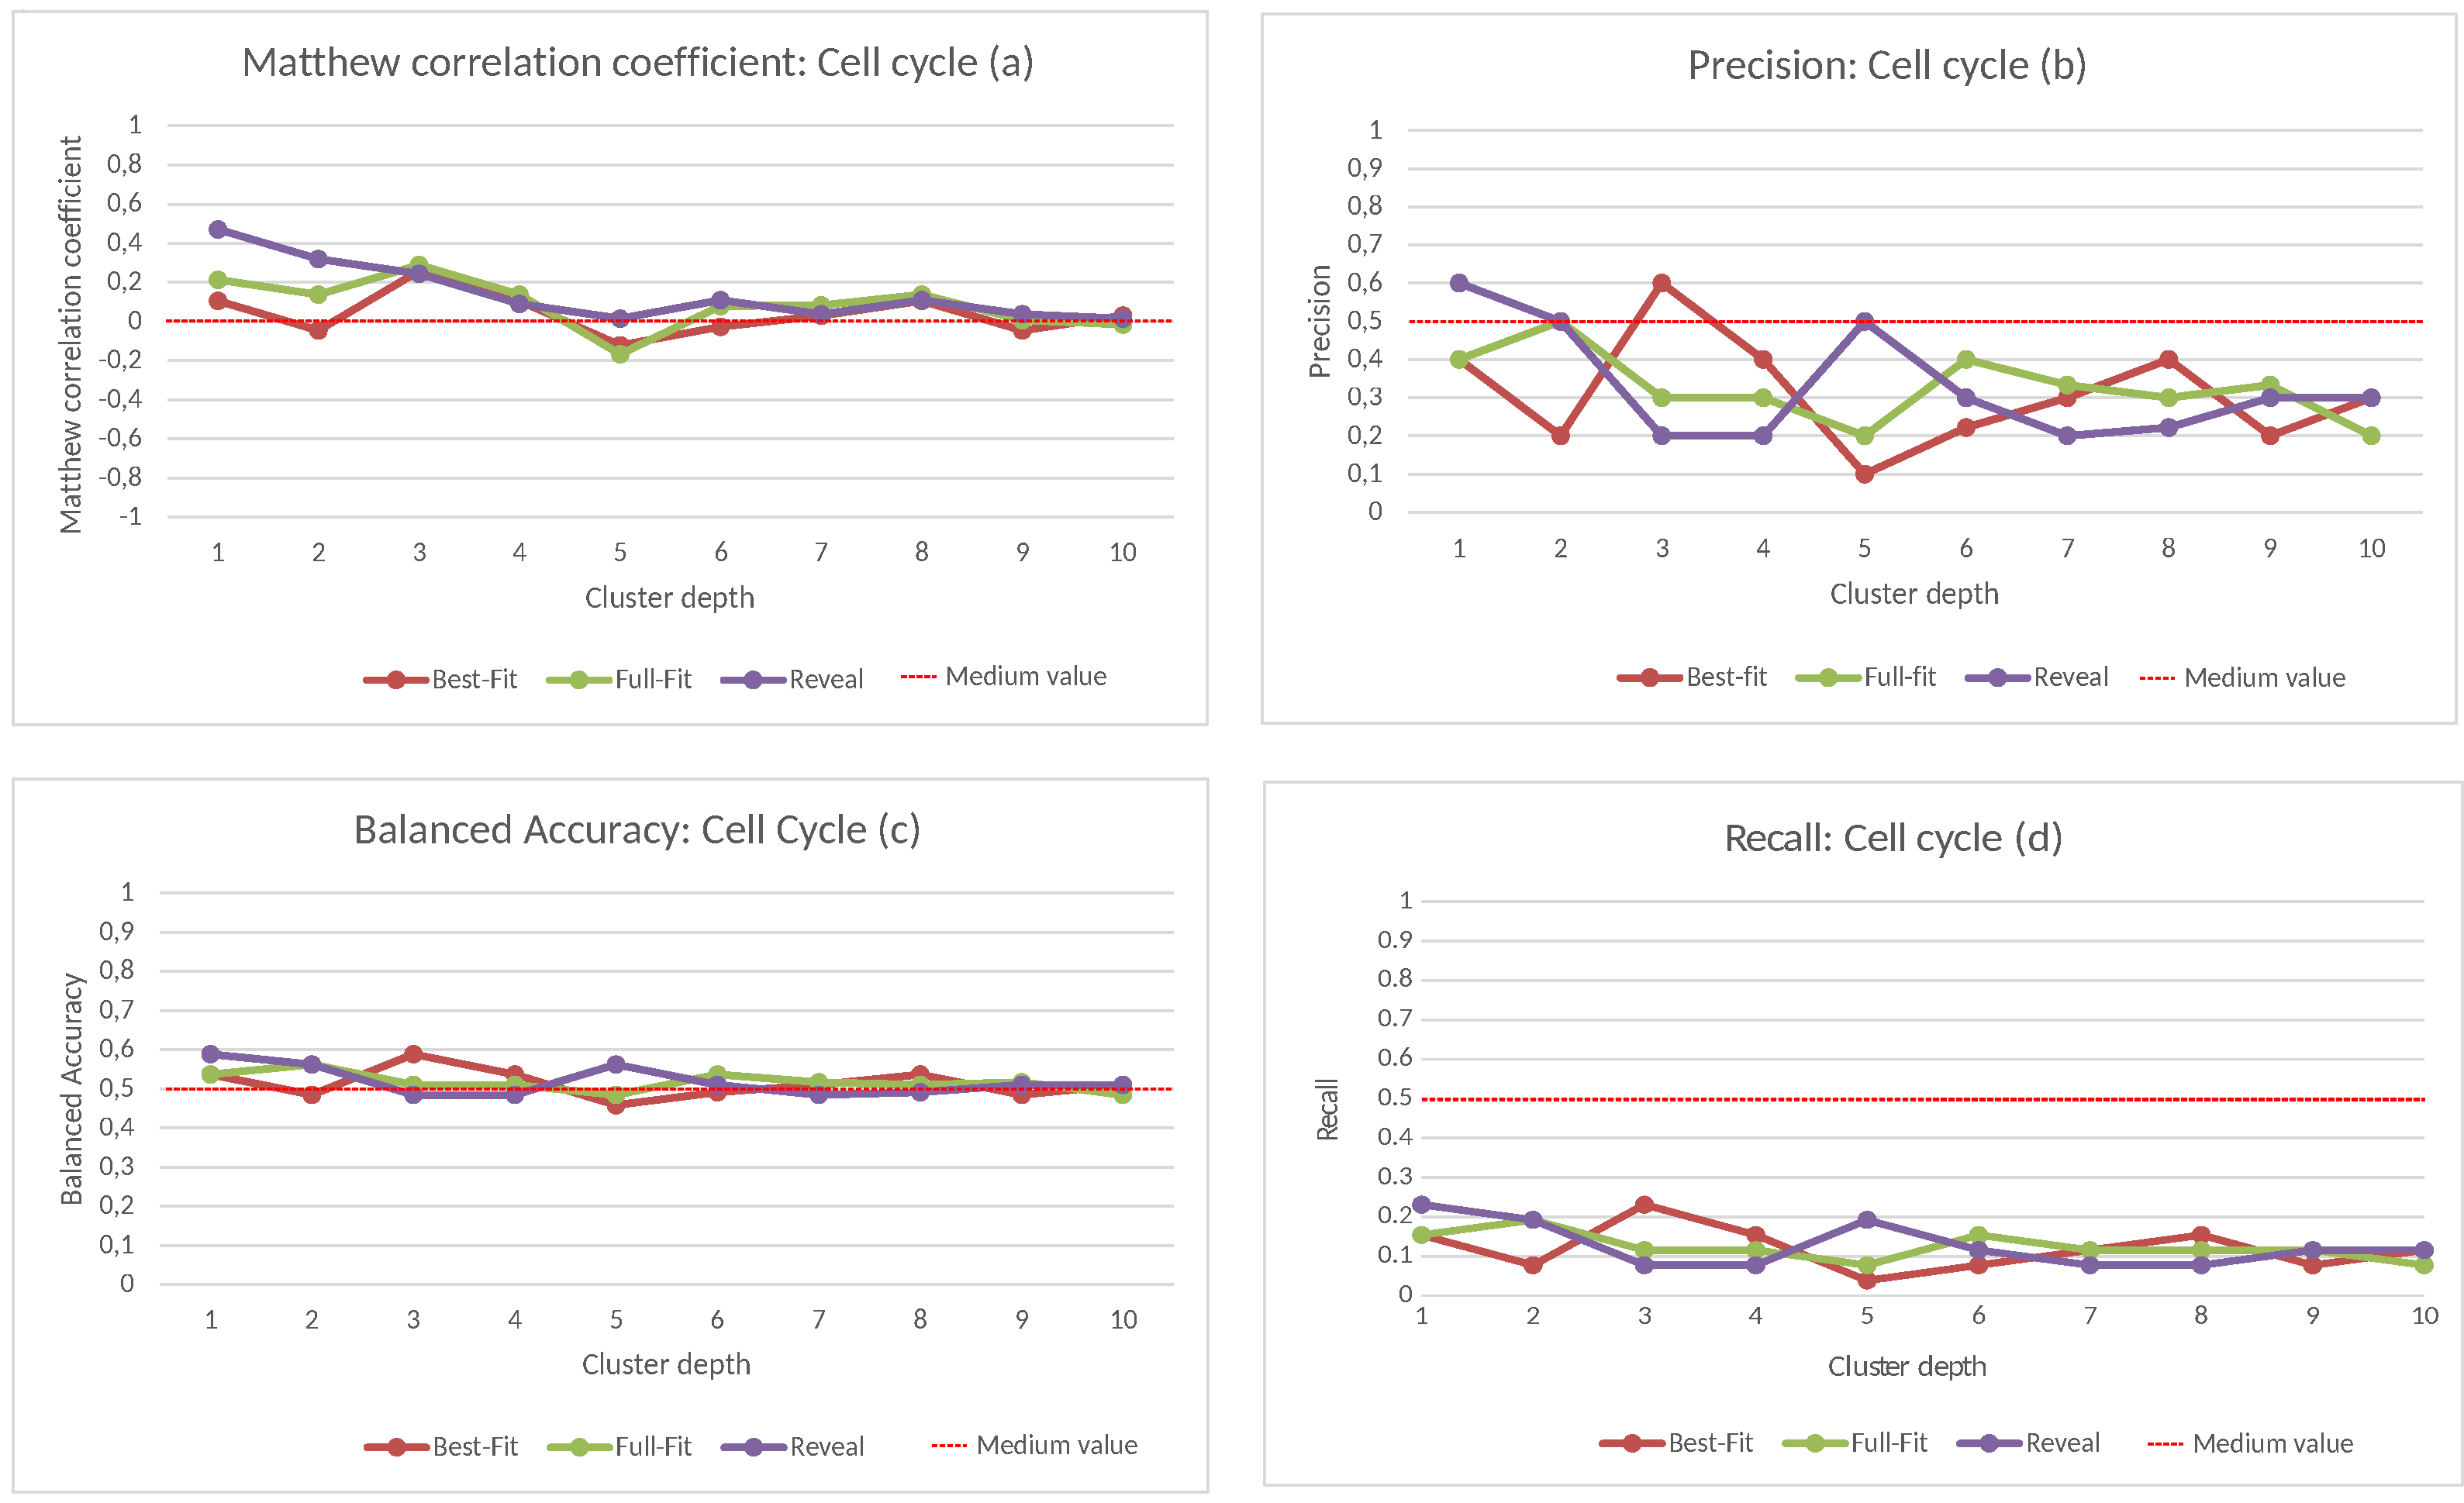
\includegraphics[width=1.0\textwidth]{./Bilder/Scoring/insilico/3_cellcycle_clusterdepth/insilico3.pdf}
\caption[Performance considering cluster depth \textit{d}]{Performance considering cluster depth \textit{d}}
\label{fig:7}
\end{figure}

Results of the performance measurement in dependence on the number of sample points are similar to the results of performance measurement in dependence on the cluster depth regarding fluctuations in precision, Best-Fit is performing the best across precision and recall and balanced accuracy and Matthew-correlation-coefficient show no outstanding performance of a method. Futhermore, regarding the runtime performance is REVEAL computuationally expensive (Figure 2.2) and therefore not an appropriate method for big real-life data network inference. Taking prior knowledge from literature into account then Best-Fit in combination with the iterative \textit{k-means} binarization algorithm captures the structural and dynamic complexity in a system the best \citep{Berestovsky.2013}.
For these reasons, this combination is applied to the real-life data set of the DREAM8-Challenge described in the next section.
%%%Wie kann man die Fluktuationen erklären????
%Diskussion:
%- MCC+BACC: TN und FN werte sind deutlich höher, daher reguliert es diese werte.
% Recall: zeigt dadurch eher, dass gerademal mean recall 9,5% der relevanten elements are selected sind und durch precision weiß, man, dass mean precision: 23,6% der selected elements sorrect sind.
%Hohe Fluktuation bei Precision: Higly oscillating system.
%\newpage
\section{Pipeline of the DREAM8 Challenge data set}
\begin{figure}[!h]
\centering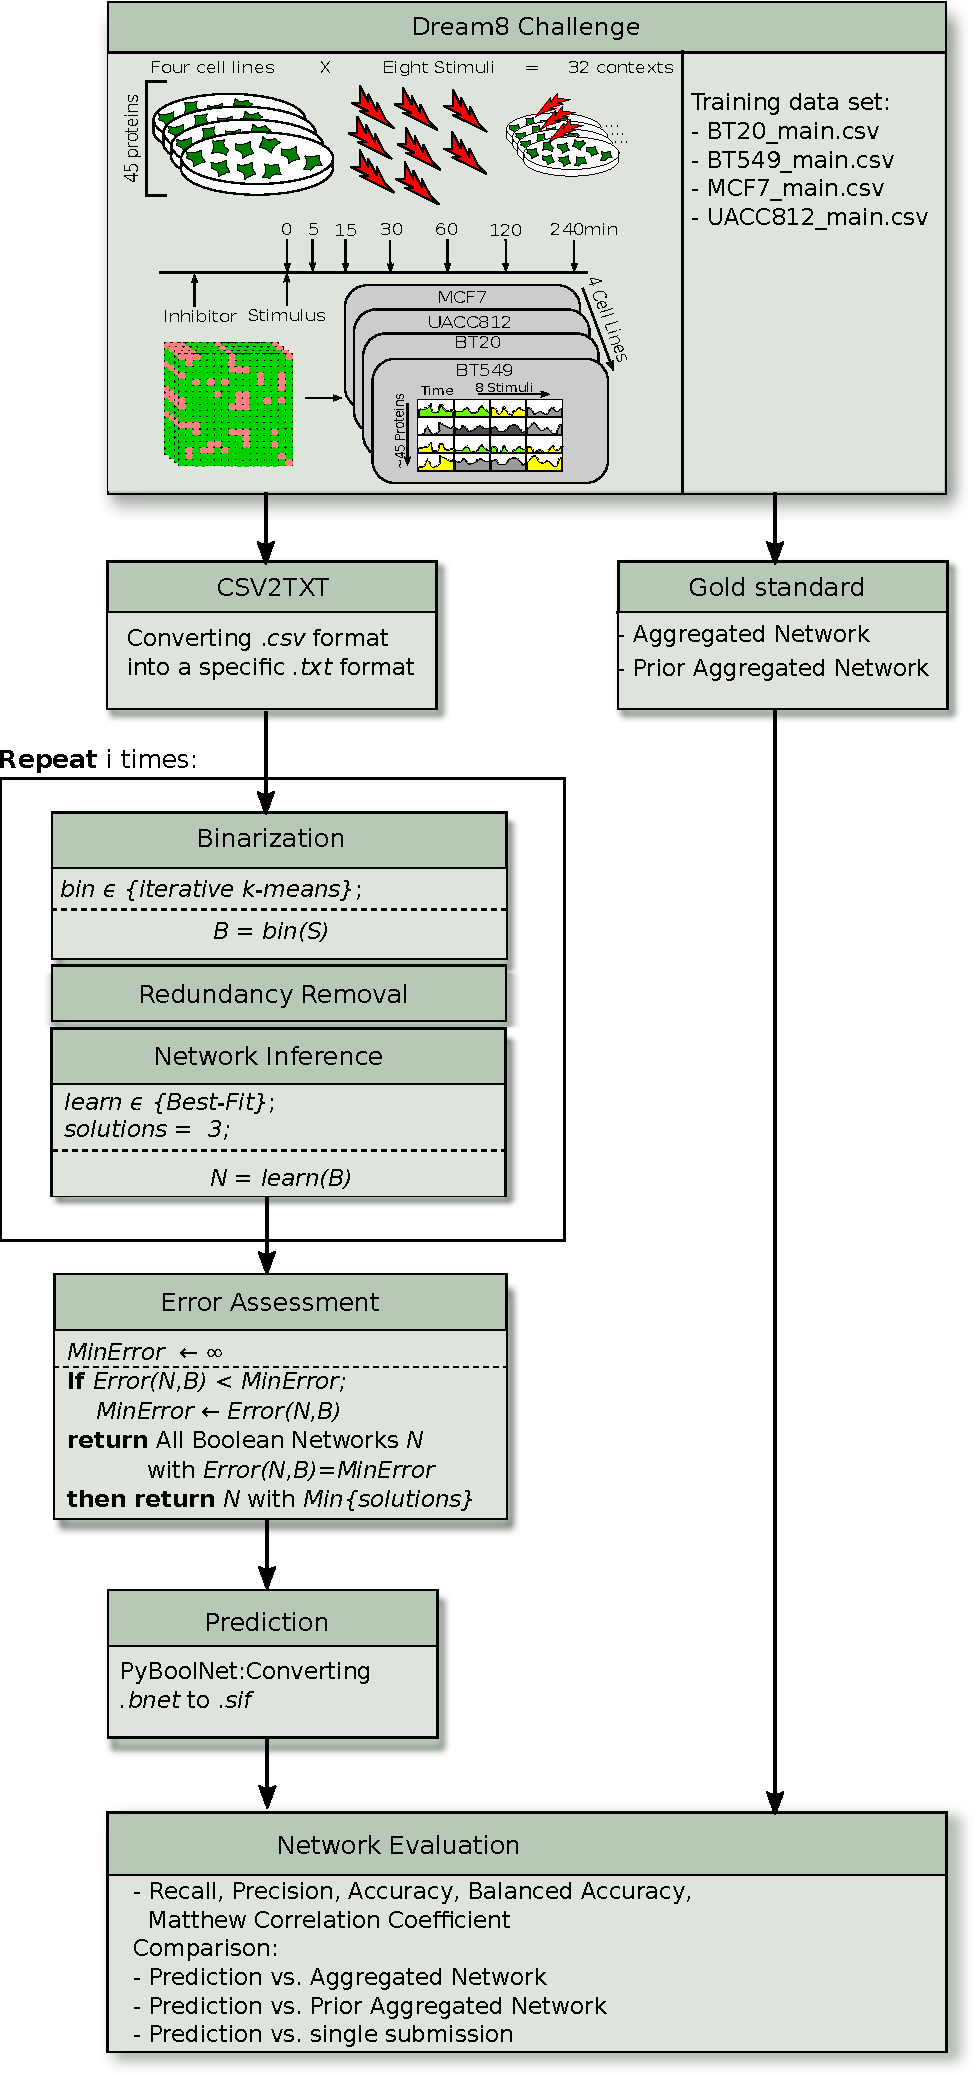
\includegraphics[width=0.6\textwidth]{./Bilder/pipeline_dream8.pdf}
\caption[Pipeline DREAM8-Challenge]{\textbf{Pipeline DREAM8-Challenge. }This pipeline shows the final setup for the DREAM8-Challenge input data. Settings are selected by previous investigation of the \textit{in silico} data set and prior knowledge from literature.}
\label{fig:9}
\end{figure}

%Threshold: Wenn ich mehrere solutions habe, dann edge score berechenen über die Häufigeit von auftretenden Kanten, dann threshold verschieben, sodass von wenig bis viele tp sich ergeben = AUROC / = AUPR (Wegen runtime nicht gemacht,aber ich dann es ja für nur 3 runs zeigen?)


%Create 32 data set from training data -> txt. file
In this section it is shown in which way the \textit{in silico} pipeline is validated, such that the DREAM8-Challenge data set can be processed, resulting in a DREAM8-Challenge pipeline depicted in Figure 3.8.\\ 
This pipeline starts with the 'main' training data set of the DREAM8-Challenge, which is converted into a \textit{txt} file format (Table 2.1, Figure 3.1) by splitting each data set of a cell line into eight text files depending on each stimulus. Each of the resulting 32 \textit{text}-files contain about $\sim 85$ sample points and about $\sim 45$ antibody names.

\subsection*{Setting selection}
%Quelle: TS2B Paper mit KM3 Empfehlung
%The python implementation of the inference algorithms is validated, such that a network up to 50 nodes can be inferred and the 
%Network inference: KM3+Best-Fit
The higher the \textit{in-degree} of each node (Figue 3.4) and the abundance of nodes in a network (Figure 2.2) the higher is the complexity in a system and hence, the higher is the computational cost of an inference algorithm \citep{Barman.2017}. 
The aim of the \textit{in silico} pipeline is to investigate which parameter has a major influence on the algorithms performance, such that the best performing algorithm can be selected for the DREAM8-Challenge data set.\\
As mentioned in 2.1 technical requirements limit (8 RAM and a Core i5 processor) the application of REVEAL to the DREAM8-Challenge data set resulting an infeasible task (Figure 2.2). This observation is confirmed by Shohang Barman and Yung-Keun Kwon \citep{Barman.2017} who state that mutual information based approaches like REVEAL are computationally expensive, because they are implemented to compute the exact mututal information values over all possible combination of nodes. Therefore, REVEAL is not considered in this pipeline.\\\\

Furthermore, results of the \textit{in silico} pipeline regarding the choice of abundance of sample points (Figure 3.6) and cluster depth (Figure 3.7 (c)) show no significant influence on the algorithms' performance. An increasing \textit{in-degree} (Figure 3.7 ) shows an decreasing performance for all three algorithms, such that no algorithm can be excluded by this investigation either.\\\\
Thus, results regarding error assessment of Best-Fit, Full-Fit and REVEAL in combination with two cluster \textit{k-means} binarization algorithm and iterative \textit{k-means} binarization algorithm of Natalie Berestovsky and Luay Nakhleh are taken into account. In this paper based on minimal error, convergence and uniqueness the recommended combination of Best-Fit with the iterative \textit{k-means} algorithm (with $d=3$) for complex systems is applied to the DREAM8 Challenge data set.\\\\%Tabelle in das supplementary,wo gezeigt wird wie gut die performance ist?
As in the \textit{in silico} pipeline the minimal error is set to a value of ????? and maximally runs 5000 times by returning 3 networks and selecting the solution with the lowest error. Predicted Boolean networks (in \textit{bnet}-format (Figure 3.2)) are converted into an interaction graph (in \textit{sif}-format (Figure 3.2)) and scored against two aggregated networks
each representing an aggregated network and an aggregated prior network each representing a gold standard.\\\\ 

For simplification of notation the prediction is defined by the set of networks predicted by the DREAM8-Challenge pipeline with the inference algorithm Best-Fit and the iterative \textit{k-means} binarization algorithm with $d=3$.


\subsection*{Gold standard and Evaluation selection}
Since gold standard networks are often based on prior knowledge from literature, learning novel connections in a network, such that specific biological systems can be truly mimicked is restricted \citep{Hill.2016}. Therefore, the DREAM8-Challenge did not provide a gold standard to the participants. Thus, a provided test data set was used as an abstracted representation of a gold standard to asses the algorithms' performance resulting in prior knowledge independent networks. \\
%Additionally an \textit{in silico} data set covering main characteristics of the experimental setting, but without batch effects, is provided by the challenge. This \textit{in silico} data set is a tool for assessing the performance of an algorithm in an idealized setting. Hence, the performance of an algorithm excluding pertubational effects can be assessed.
%The \textit{in silico} data set is generated from a non-linear ordinary differential equations (ODE) model of the ERBB signalling pathway (ERBB:family of proteins containing four receptor tyrosine kinases, structurally related to the epidermal growth factor receptor (EGFR)). Nevertheless pre-existing biological knowledge was included by several participants and seemed to be broadly beneficial.\\
%Warum beneficial? Zeigen, dass die performance der gruppen mit prior knowledge nicht signifikant schlechter war als bei gruppen ohne

%Evaluation in the DREAM8-Challenge
Due to varying strategies of evaluating predictions, e.g. choice of the scoring metric and implementation strategy, it is quite challenging to compare the resulting performances between the participants reliably. For this reason the DREAM8-Challenge provides a standard scoring tool: 'DREAMTools' python package \citep{Cokelaer.2015}.\\
This tool needs as input a \textit{sif}-file and an \textit{eda}-file, while an \textit{eda} (electronic design automation) contains information of edge occurrences in a network like in a \textit{sif}-file and additionally a confidence score for each edge. A confidence score (resp. edge weight) describes the probabilty of an edge being existent or not \citep{authornamenotavailable.}.\\ 

DREAMTools compares the confidence scores of a predicted network against confidence scores of a gold standard network returning values of the Area Under the Receiver Operating Characteristic curve (AUROC) and the Area Under the Precision Recall Curve (AUPR) \citep{Cokelaer.2015} \citep{Hill.2016}. Both evaluation metrics are commonly used when there is an imbalance between the number of positives and negatives in the gold standard \citep{Davis.2006}.
For further details regarding definition and application of these metrics the reader is referred to section A.1.'DREAM8-Challenge scoring priciples'. In subchallenge SC1A of the DREAM8-Challenge each participating group was ranked by their scoring results, revealing which inference performs the best \citep{authornamenotavailable}.\\\\

In contrast to the DREAM8-Challenge this work makes use of an aggregated network and an aggregated prior network each representing a gold standard. These networks were submitted after finishing the challenge in 2016. The aggregated network is a compendium of 66 submissions of the participants with the best performance reduced by correlated submissions \citep{Hill.2016}. Thus, this network comprises prior knowledge networks with prior knowledge independent networks.
The aggregated prior network is a combination of 10 prior knowledge networks that participants used as part of their submission \citep{Hill.2016}.
Table 3.2 gives an overview of the properties of the aggreagted network, aggregated prior network and the prediction reagarding the number of nodes and links in each network and the number of networks each network is composed are shown.

\begin{table}[H]
%\resizebox{\textwidth}{!}{
%{\tabcolsep=6pt%
\begin{center}
%\captionsetup{width=0.87\linewidth}
%\small
\begin{tabular}{l|c|c|c}
\toprule 
Network & $\# $ nodes & $\# $ edges & $\# $ networks\\
 \hline\hline
Prediction (Best-Fit) & $\sim 45$ & $\sim 140$ & 1\\
\rowcolor{black!10} Aggregated Network & $\sim 45$ & $\sim 2200 $ & 66\\
Aggregated Prior Network & $\sim 45$ & $\sim 1400$ & 10\\
\bottomrule
\end{tabular}
\captionof{table}{Network properties}
\end{center}
%}
\end{table} 

Predictions of all 74 participating groupes of the DREAM8-Challenge for the SC1A challenge and the prediction generated by the DREAM8-Challenge pipeline are scored against the aggregated network and against the aggregated prior network. This results in a new ranking including the pipelines' prediction, revealing how a Boolean approach is performing in relation to the participants' submission.\\\\ 
Instead of taking AUPR and AUROC, balanced accuracy, Matthew correlation coefficient, precision and recall are implemented in this pipeline. 

\newpage
\section{Results of the DREAM8-Challenge data set}

In this section first it is emphasized why it is recommanded to use balance accuracy instead of accuracy for an imbalanced set. Then the prediction and all submissions of the DREAM8-Challenge are ranked by scoring these networks against the aggregated network and aggregated prior network. 

\subsection*{Prediction versus Aggregated Network and Aggregated Prior Network}

In Figure 3.9 the prediction is scored against the aggregated network and the aggregated prior network among the stimuli for each cell line opposing balanced accuracy to accuracy. The mean accuracy of scoring the prediction against the aggregated network yields a value of $\sim 0.126$ and for scoring the prediction against the aggregated prior network yields a value of $\sim 0.386$. The mean balanced accuracy value for scoring the prediction against the aggregated network is $\sim 0.505$ and for scoring the prediction against the aggregated prior network is $\sim 0.495$. Regarding the major distance between accuracy and balanced accuracy it is observed that the data is class imbalanced. Especially for the case of the scoring the prediction against the aggregated prior network. 

\begin{figure}[H]
\captionsetup{width=0.9\linewidth}
\centering
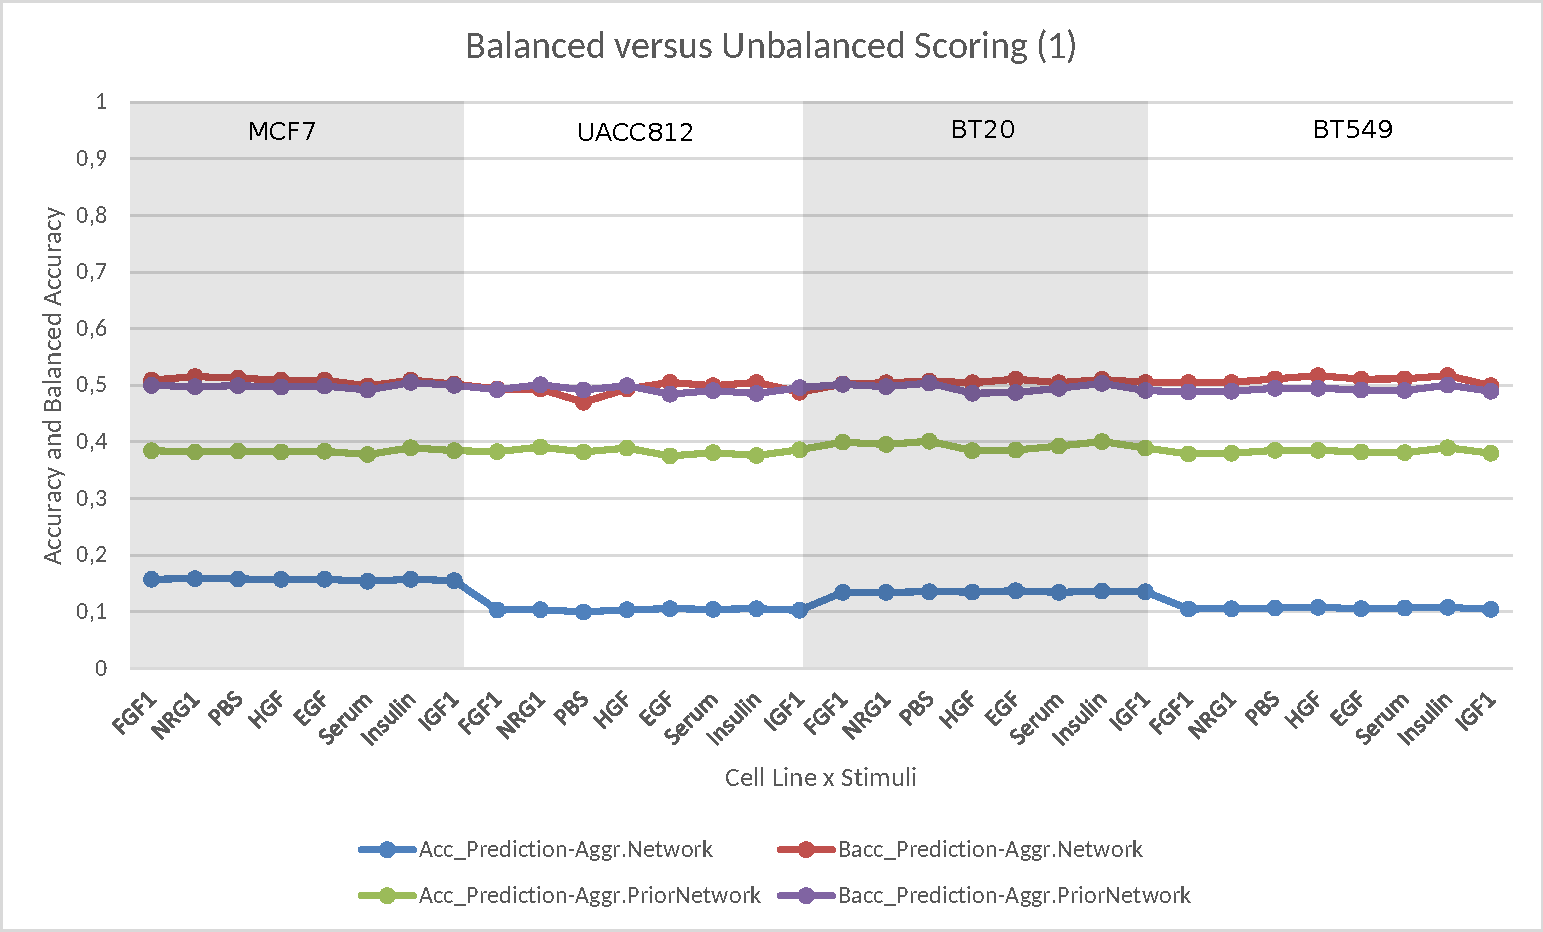
\includegraphics[width=0.9\textwidth]{./Bilder/Scoring/dreamchallenge/1_Balanced_vs_Unbalanced/balanced1.pdf}
\caption[Imbalanced classes (1)]{Imbalanced classes (1). Accuracy and Balanced Accuracy for the prediction scored against the aggregated network and aggregated prior network.}
\label{fig:10}
\end{figure}

This observation is emphasized by considering the size of each class in the confusion matrix for both evaluation measurements. Comparing the prediction with the aggregated network predominantly many false negatives are detected, thus the accuracy is worse. Whereas comparing the prediction with the aggregated prior network the number of false negatives is much lower and the number of true negatives is much higher such that the accuracy yields better result. \\\\

For emphasizing this observation the prediction is scored in Figure 3.10 instead against the aggregated prior network against a submission of the last participant (rank: 74., $\sim 600$ edges among the 32 contexts) of the DREAM8-Challenge leader board \citep{authornamenotavailable}. Here, scoring the prediction against the last participant shows that the disparity of the size between these networks is not that big as between the prediction and the aggregated network. Thus scoring the prediction against the last participant results in a predominant abundance of true negatives thus the mean accuracy of $\sim 0.716$ is much better than scoring the prediction against the aggregated network.

\begin{figure}[H]
\captionsetup{width=0.9\linewidth}
\centering
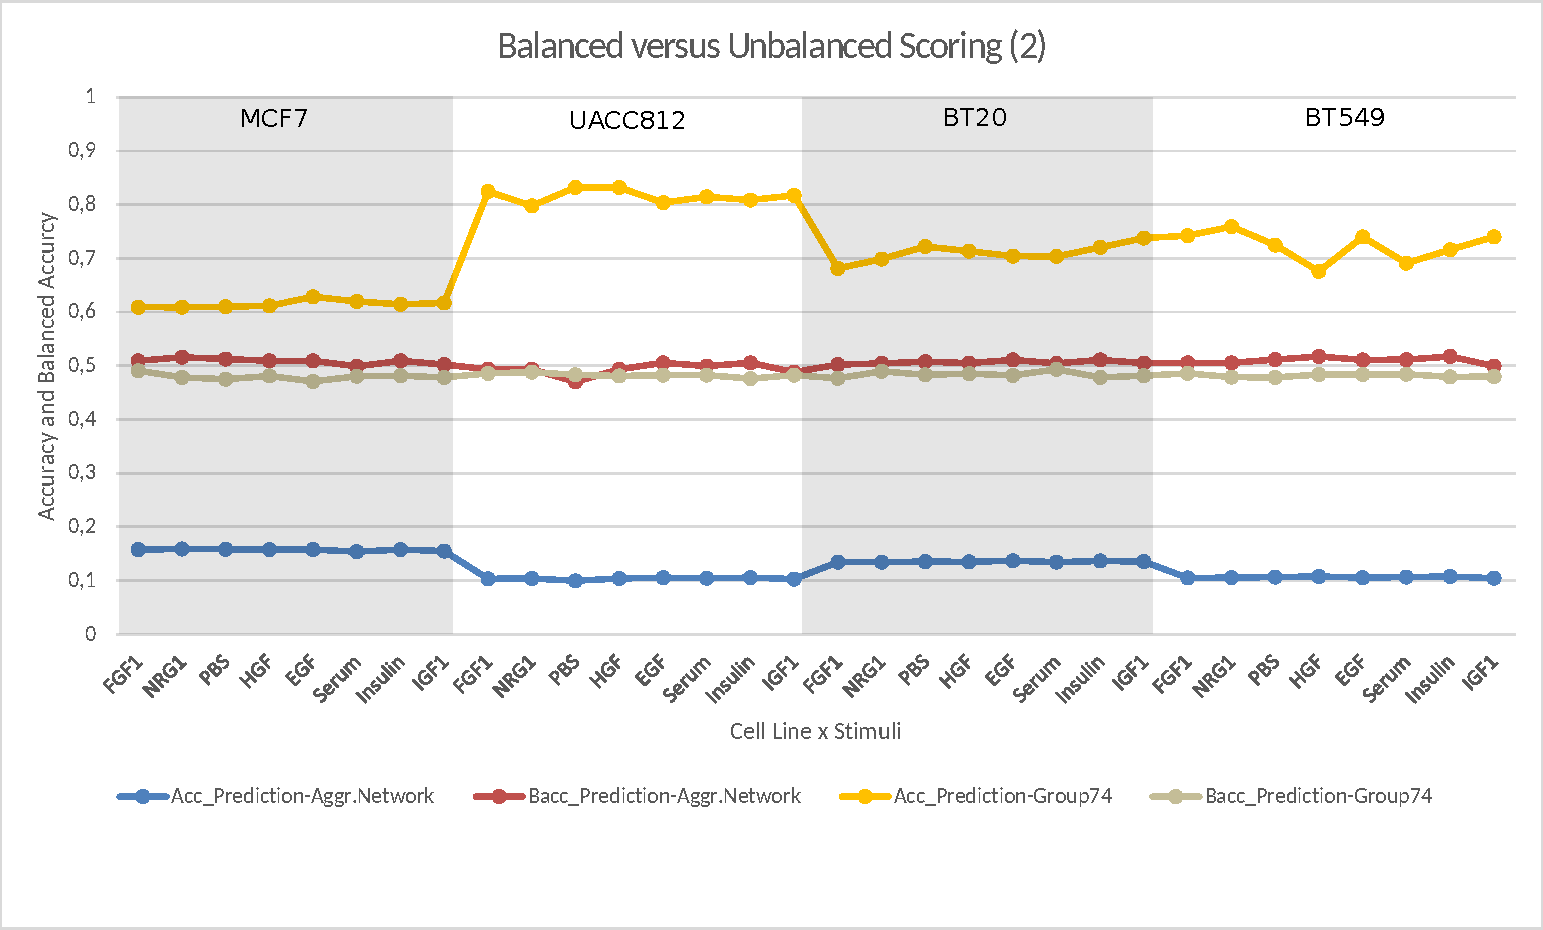
\includegraphics[width=0.9\textwidth]{./Bilder/Scoring/dreamchallenge/1_Balanced_vs_Unbalanced/balanced2.pdf}
\caption[Imbalanced classes (2)]{Imbalanced classes (2). Accuracy and Balanced Accuracy for the prediction scored against the aggregated network and aggregated prior network.}
\label{fig:10}
\end{figure}

The impact of true negatives and false negatives can be put into perspective by applying the balanced accuracy metric. Therefore accuracy is neglected and further evaluation are perfomed with precision, recall, balanced accuracy and matthew correlation coefficient.\\


In Figure 3.11 the recall (a) and the precision (b) values are shown. It is important to indicate that the recall is presented in a higher resolution such that each evaluation is easier to distinguish.\\


\begin{figure}[H]
\captionsetup{width=0.9\linewidth}
\centering
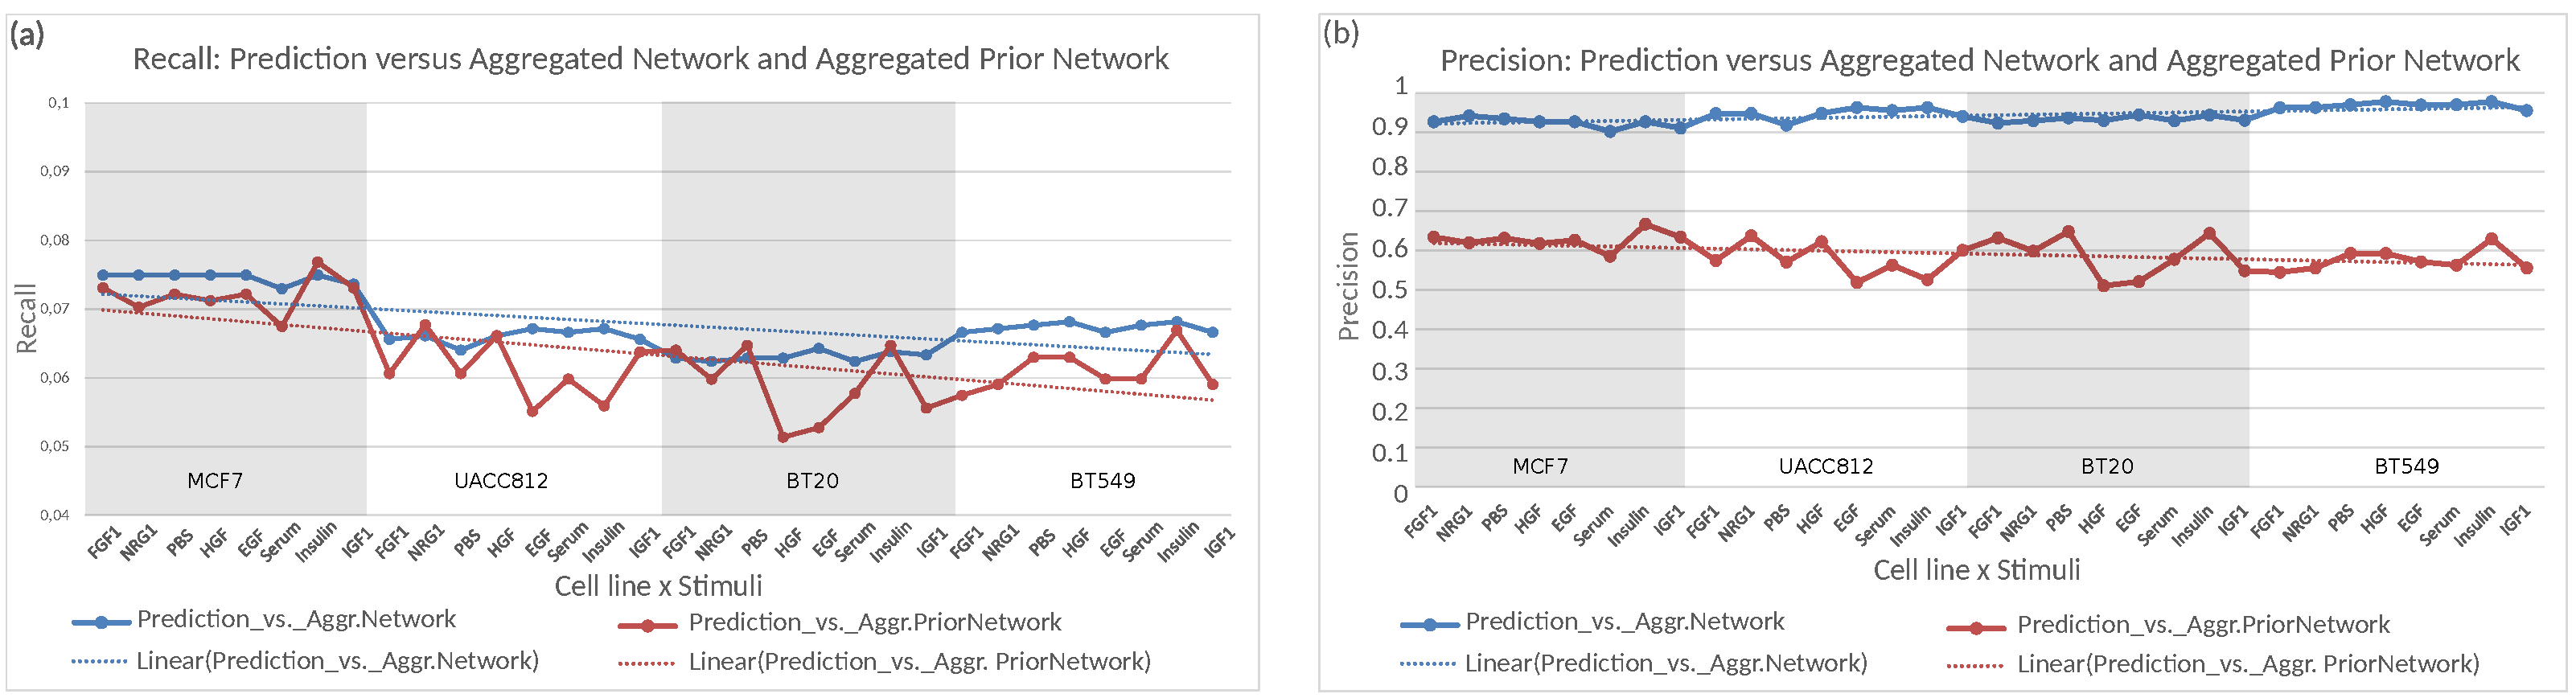
\includegraphics[width=1.0\textwidth]{./Bilder/Scoring/dreamchallenge/1_Balanced_vs_Unbalanced/balanced_recprec.pdf}
\caption[Recall: Prediction versus Aggregated/Prior Network]{Recall: Prediction versus Aggregated/Prior Network}
\label{fig:10}
\end{figure} 

In (a) the prediction is scored against the aggregated network yielding a mean recall value of $\sim 6,7\%$ and scored against the aggregated prior network resulting in a mean recall value of $\sim 6,3\%$. Beside the fact that scoring against the aggregated prior network causes a few fluctuations among cell lines and stimuli the overall mean recall value is not significantly different to the mean recall value of scoring the prediction against the aggregated network. All in all, the prediction predicted $\sim 6,5\%$ of the releveant elements.\\
In (b) the prediction scored against the aggregated network yields a mean precision value of $\sim 0.943$, meaning about $\sim 94,3\%$ edges are predicted correctly. Regarding the prediction beeing scored against the aggregated prior network regarding the mean precision value about $\sim 59,1\%$ edges are predicted correctly. 
%The aggregated network is much bigger than the prediction and much bigger than the aggregated prior network (Table 3.2). Thus, the aggregated network builds a bigger intersecting set of true values covering most of the predicted elements.

\subsection*{New Ranking: Aggregated Network and Aggregated Prior Network}

A total of $74$ submissions of participants of the DREAM8-Challenge in combination with the predicted network of the DREAM8-Challenge pipeline are scored against the aggregated network and the aggregated prior network. The networks are ranked by their mean value of balanced accuracy, Matthew correlation coefficient (Mcc), precision and recall such that a ranking of the prediction is achieved. 

In Figure 3.12-3.14 names of the participating groups of the DREAM8-Challenge are pseudonymized by their original ranking of the SC1A leaderboard.
%\citep{https://www.synapse.org/#!Synapse:syn2289138}. 
%Im Anhang Leaderboard 
For this reason the prediction of the DREAM8-Challenge is pseudonynomized by a value of $0$, which is highlighted in each figure by a red rectangle. In Table 3.3. the ranking of the prediction for each evalutaion method and its corresonding value is shown.


\begin{table}[H]
\begin{center}
%\captionsetup{width=0.87\linewidth}
%\scriptsize
\small
\begin{tabular}{l|c|c|c}
\toprule 
\textbf{Scoring metric} &\textbf{Type} & \textbf{Aggregated Network} & \textbf{Aggregated Prior Network}\\
 \hline\hline
\rowcolor{black!10} Mean Balanced Accuracy & rank & 43 & 49\\
  & value & $\sim 0.0628$ &$\sim 0.4950$\\
\rowcolor{black!10} Mean Mcc & rank & 33 & 39\\
  & value &$ \sim 0.0097$ &$ \sim 0.0195$\\
\rowcolor{black!10} Mean Precision & rank & 33 & 45 \\
 & value & $\sim 0.9436$& $\sim 0.5909$\\
\rowcolor{black!10}Mean Recall & rank & 42 & 47\\
  & value & $\sim 0.0677$ & $\sim 0.0632$\\
\bottomrule
\end{tabular}
\captionof{table}{Ranking of the prediction}
\end{center}
%}
\end{table} 

In Figure 3.12 mean balanced accuracy values are descend ordered by the values of all submissions and the prediction scored against the aggregated prior network. In relation to the DREAM8-Challenge submissions the prediction has a rank of 49 with a value of $\sim 0.495$. Mean balanced accuracy values ordered by the aggregated network yields a rank of 43 for the prediction with a value of $\sim 0.063$.\\%Grund: FN so immens hoch, sodass selbst BACC das nicht mehr relativieren kann.
Regarding the mean Matthew-correlation-coefficient in Figure 3.13 the networks are descend ordered by the results of scoring against the aggregated network. For this case the prediction yields a new rank of 33 with a value of $\sim 0.0097$ and values ordered by scoring against the aggregated prior network yield a rank for the prediction of 39 and a corresponding value of $\sim 0.0195$.


Regarding the mean recall ranking in Figure 3.13 the ranking is ordered by the scoring against the aggregated prior network, and the prediction predicts $\sim 6,8\% $ of relevant edges of the aggregated network with a rank of 42 and predicts $\sim 6,3\% $ of relevant edges of the aggregated prior network with a rank of 47.\\ 
Furthermore, the precison shows that regarding the aggregated network the prediction predicts $\sim 94.36\%$ of the relevant edges correctly with a rank of 33 and regarding the aggregated prior network the prediction predicted $\sim 59,1\% $ of the relevant edges correctly with a rank of 45.\\\\ 

Averaging across the whole evaluation set for scoring against the aggregated network the prediction  yields a rank of 49 and for scoring against the aggregated prior network the prediction yields a rank of 50.
It is noticed that averging among the whole evaluation set captures the ranking of the best performing group in the DREAM8-Challenge. This control emphasizes the reliability of evaluation methods used in this thesis.

% Balanced Accuracy
\begin{figure}[H]
\centering
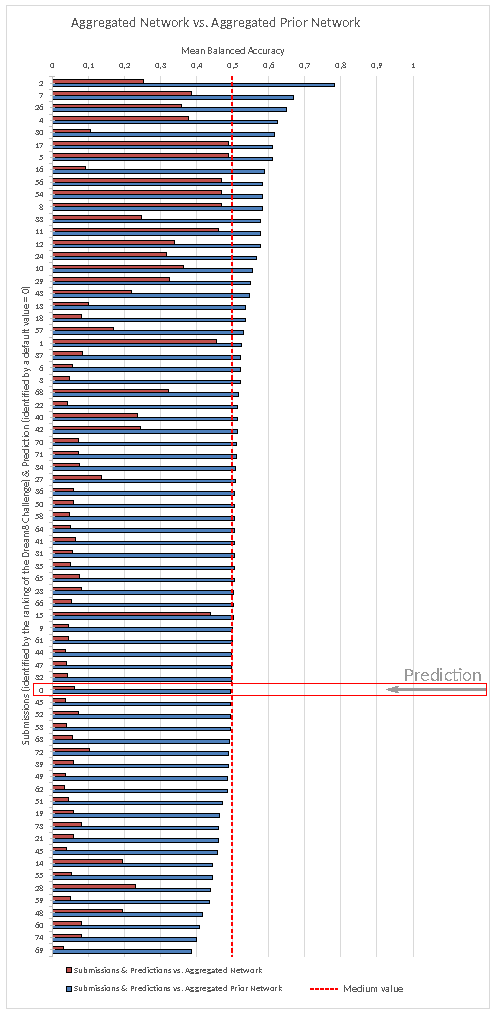
\includegraphics[width=0.7\textwidth]{./Bilder/Scoring/dreamchallenge/Meanbacc_vertical_comparison2.pdf}
\caption[New Ranking Balanced Accuracy]{New Ranking (Balanced Accuracy): Aggr. Network and Aggr.Prior Network}
\label{fig:}
\end{figure}


%MCC
\begin{figure}[H]
\centering
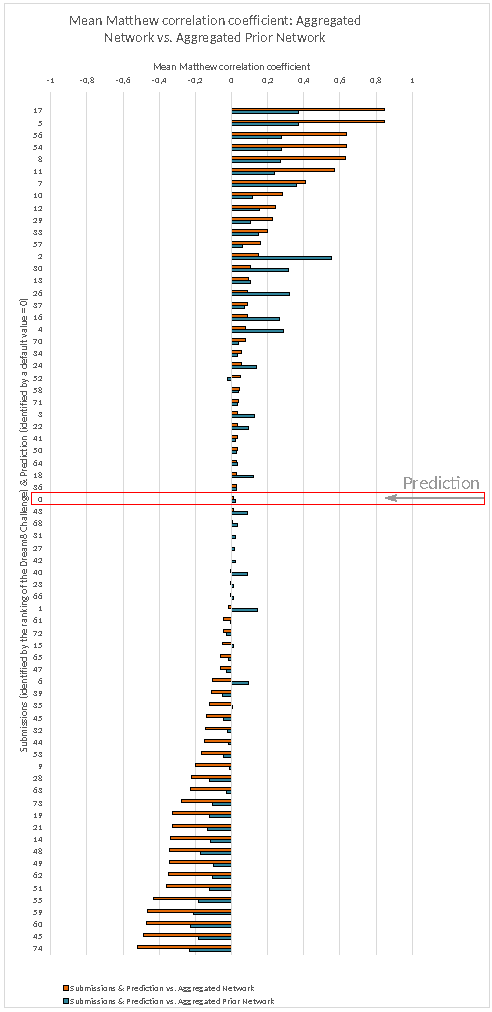
\includegraphics[width=0.7\textwidth]{./Bilder/Scoring/dreamchallenge/MeanMcc_vertical_comparison2.pdf}
\caption[New Ranking: Matthew correlation coefficient]{New Ranking (Matthew correlation coefficient): Aggr. Network and Aggr.Prior Network}
\label{fig:}
\end{figure}

%Precision and Recall
\begin{figure}[H]
\centering
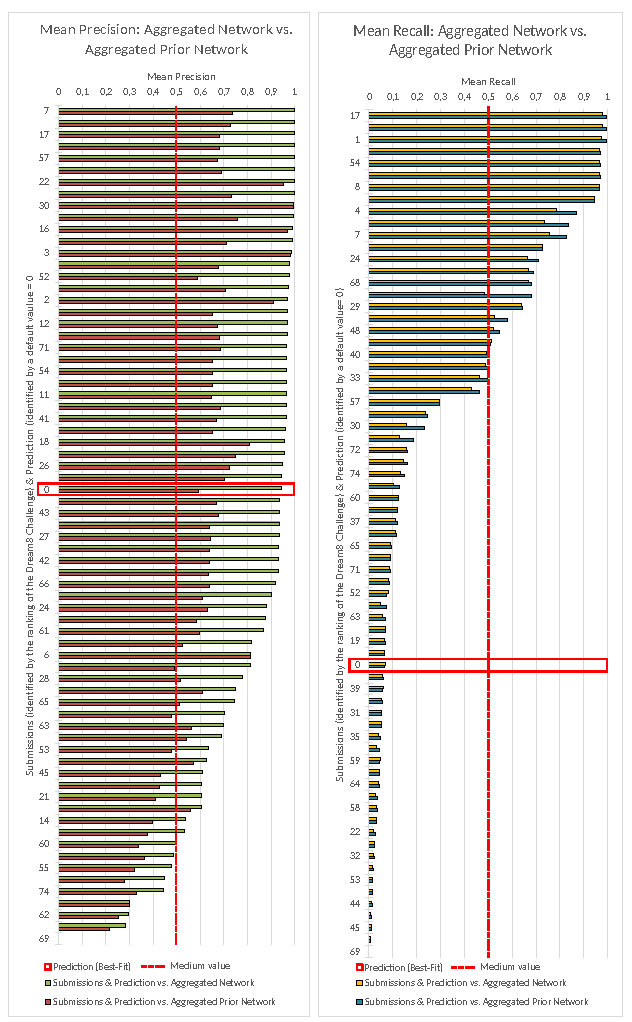
\includegraphics[width=0.82\textwidth]{./Bilder/Scoring/dreamchallenge/Recall_Precision_vertical_comparison.pdf}
\caption[New Ranking: Precision and Recall]{New Ranking (Precision and Recall): Aggr. Network and Aggr.Prior Network}
\label{fig:}
\end{figure}





